\documentclass{article}
\usepackage{enumitem}
\usepackage{authblk}
\usepackage{graphicx}
\usepackage{fullpage}
\usepackage[font=small,labelfont=bf]{caption}
\usepackage{tikz}
\usetikzlibrary{trees}

\begin{document}  
\title{CSPy Ulysses Documentation For Teacher And Student Usage} 
\author{Paul Magnus '18, Ines Ayara '20, and Matthew R. Jenkins '20, advised by Alistair Campbell}
\maketitle{}

\tableofcontents

\newpage

\section{Introduction} 
This is the documentation for CSPy, a strongly-typed Python dialect for use in learning environments. This is the Ulysses version, which is the third version of the dialect. It succeeds the Jabberwocky version made by Lyndsay LaBarge '17 and Maya Montgomery '18, which is itself preceded by a foundation written by Alex Dennis '18 and Eric Collins '17. We thank those responsible for earlier versions for making our lives easier and providing a suitable framework for our improvements. 

\subsection{What is CSPy?}
CSPy is a strongly-typed dialect of Python. Python by itself is not strongly typed and because of this, new programmers that use Python can use it in bad ways, like creating variables that end up not being used, or by setting a variable of a specific type to another type. With CSPy, we are more up front about these problems. Any things have to be named at the start of each function definition or class definition or program, and CSPy makes sure each thing is used and is not changed to a different thing by the writer. These things make it easy to teach future programmers about programming languages, and helps to make learning other object oriented programming languages easier in the future.

\subsection{How To View And Use This Document}
This document should give a decent primer for how to teach an introductory course in Computer Science. It discusses the grammar rules of the CSPy dialect, how to initalize variables, how to create classes, what counts as a function/procedure, what counts as an expression, what counts as a statement, and contains appendices of all built in functions and types. It is mostly meant as a reference, not as a teaching aide.

The authors advise against printing out this document, as it is lengthy and generally not designed for print form. If you have to print this document, print double sided. This document is rendered using \LaTeX.

\subsection{Contact Information}
Please send CSPy and graphical environment issues to pmagnus@hamilton.edu, any issues related to the CSPy editor to iayara@hamilton.edu, and any documentation and graphical environment issues to mjenkins@hamilton.edu. We will be happy to fix anything you find. If any of us are unable to be reached, please email acampbel@hamilton.edu and he'll forward any issues to us.

\pagebreak

\section{CSPy Grammar Rules}
\subsection{The Basics}
Each variable declared in CSPy has to be declared in the following format, at the beginning of each function or class definition: \\

\verb|::NAME:TYPE::| \\

\verb|NAME| can be any name so long as it starts with a to z/A to Z (meaning you can't start it with a number or underscore, but you can put numbers or underscores anywhere else in the name - just like Python), but \verb|TYPE| has to be named after an object type:

\begin{itemize}
\item \verb|TYPE:int| - any integer (eg. \verb|7|) 

\item \verb|TYPE:float| - any decimal representation of a number (eg. \verb|5.6|) 

\item \verb|TYPE:bool| - \verb|True| or \verb|False| 

\item \verb|TYPE:string| - 
\verb|"Hello, world!", 'Hello, world!'| \\ (NOTE: These CANNOT include new lines.) 

\item \verb|TYPE:string| - 
\verb|"""Hello, world!""", '''Hello, world!'''| \\ (NOTE: These CAN include new lines.) 

\item \verb|TYPE:list of TYPE| - \verb|[1, 2, 3, 4]| 

\item \verb|TYPE:[TYPE]| - \verb|[1, 2, 3, 4]| \\ (NOTE: The form \verb|[TYPE]| is an alternate form, and can be useful when making a list of lists.) 

\item \verb|TYPE:tuple of (TYPE * TYPE * ...)| - \verb|("A", 1)| 

\item \verb|TYPE:(TYPE * TYPE * ...)| - \verb|("A", 1)| \\
(NOTE: The form \verb|(TYPE * TYPE * ...)| is an alternate form, and can be useful when making a tuple of tuples or a nested list of tuples.) 
% Needed | symbol within printed expression
\item \verb!NAME:dict of [KEY | VALUE]! - \verb|{1:"a", 2:"b"}| 

\item \verb|TYPE:set of TYPE| - \verb|{5, 6, 7, 8}| \\
(NOTE: \verb|{}| is an empty dictionary. To make an empty set, use \verb|makeset()|.)

\item \verb|TYPE:frozenset of TYPE| - \verb|{5, 6, 7, 8}| \\ 
(NOTE: \verb|{}| is an empty dictionary. To make an empty frozenset, use \verb|frzset()|.)

\item \verb|TYPE:generator of TYPE| \\
(NOTE: Generators can only be created from functions in CSPy that contain a yield statement. See \ref{generators_and_yield} on page \pageref{generators_and_yield} for more information.)

\item \verb|TYPE:file| - Type returned by the built in function \verb|open()|.

\item \verb|TYPE:fn (p1, p2, ...) -> r| - Function whose first parameter has type \verb|p1|, second parameter has type \verb|p2|, etc. and whose return type is \verb|r|.

\item \verb|TYPE:proc (p1, p2, ...)| - Process whose first parameter has type \verb|p1|, second parameter has type \verb|p2|, etc. and does not return anything. 
\end{itemize}

More details on types can be found in Appendix 1.
\subsection{Classes}
If you make a class, then the type has to be named after that class. For example, if there is a \verb|class Circle|, an object has to be named like so: 

\begin{itemize}
\item \verb|NAME:Circle|
\end{itemize}

Variables of a Class type can equal an object made from that class or they can equal \verb|None|, which means it equals no object. Only classes can equal \verb|None|. If any other type is set to \verb|None|, a TypeError will be thrown.

A sample declaration of \verb|class Circle| is as follows:
\begin{verbatim}
class Circle:
    :: center:tuple of (int * int), radius:int ::
    def Circle(x:int, y:int, r:int):
        center = (x, y)
        radius = r

    def area(c:Circle) -> float:
        return (3.14 * (c.radius ** 2))
\end{verbatim}
The variables in between the class declaration and the class methods are public attributes of the class. Anything put there is only used in the scope of the class, but can be accessed through dot syntax, such as \verb|c.center| or \verb|c.area(d)| (assuming \verb|c| and \verb|d| are both of type \verb|Circle|). Within any class definition, the variable \verb|self| is defined to be the class instance itself. Although this is not needed in most cases, \verb|self| can be used as a parameter to functions or to differentiate between class varables and local method variables. In CSPy, \verb|self| works similarly to how \verb|this| is used in Java.

Each constructor has to be named after the class name. The constructor is only executed once (at the creation of each object), and does not return anything. In this case, \verb|Circle(int, int, int)| is the constructor for the class \verb|Circle|.

The method \verb|area(c:Circle)| takes an object of type \verb|Circle| as a parameter. Classes are allowed to have local variables in their methods whose types correspond to the class being defined.

Classes can have super classes:
\begin{verbatim}
    class Circle extends Shape:
\end{verbatim}
In this case, \verb|Shape| is the super class of \verb|Circle|. All of \verb|Shape|'s methods can be used within \verb|Circle|.

Classes can have both constructor overloading and method overloading, so long as each formal parameter list is distinct from others in the class. For example, our \verb|Circle| class can have two or more constructors:
\begin{verbatim}
class Circle:
    :: center:tuple of (int * int), radius:int ::
    def Circle(x:int, y:int, r:int):
        center = (x, y)
        radius = r

    def Circle(c:tuple of (int * int), r:int):
        center = c
        radius = r
    ......
\end{verbatim}

Methods can be overloaded as well:
\begin{verbatim}
class Circle:
    :: center:tuple of (int * int), radius:int ::
    ......
    def area(c:Circle) -> float:
        return (3.14 * (c.radius ** 2)) 

    def area() -> float:
        return (3.14 * (radius ** 2)) 
\end{verbatim}

\subsection{Functions and Procedures}
CSPy differentiates between Functions and Procedures. Functions must return something of the type specified, but procedures do not return anything.

The types of each variable in a formal parameter list must be declared, and if an object is returning anything it has to be indicated through \verb|->| syntax. Anything returned must match the type after the \verb|->|:
\begin{verbatim}
    def add(x:int, y:int) -> int:
        return x + y

    def add(x:float, y:float) -> float:
        return x + y
\end{verbatim}

Function overloading is supported in CSPy, but only if each formal parameter list is distinct from others. Changing the return type does not make the function different:
\begin{verbatim}
    def add(x:int, y:int) -> float:
        return tofloat(x + y)
\end{verbatim}
If this was in the same \verb|.cspy| file as the above two functions, the program would not run because it would detect a duplicate class and throw an exception.\\

Procedures can be overloaded as well, provided that each procedure's parameter list is different:
\begin{verbatim}
    def output(x:int):
        print(x)

    def output(x:float):
        print(x)
\end{verbatim}

\subsubsection{Generators and Yield} \label{generators_and_yield}
CSPy generators function similarly to Python generators. The type \verb|generator| in CSPy is an iterator of arbitrary length. Within CSPy generators can only be created from a function using the \verb|yield| statement.
\begin{verbatim}
    def short_generator() -> generator of int:
        ''' This function creates a generator of a
            short list of integers '''
        for x in [4, 3, 7, 0, 3]:
            yield x
        raise StopIteration

    def int_generator() -> generator of int:
        ''' This function creates a generator of all
            positive integers in sequence '''
        :: x : int = 0 ::
        while True:
            x = x + 1
            yield x
        raise StopIteration
\end{verbatim}
All CSPy generators must end with \verb|raise StopIteration| even if they are infinite generators as shown in the second example. As with any 'infinite' object in a computer, caution should be taken in order to avoid an unending program.

\subsection{Loops and Conditionals}
For loops retain the same syntax as Python. The only thing that can't be done is iteration over a tuple, because they can have values of different types within them. Being able to do this clashes with CSPy's strong typed nature, so it is better if CSPy forbids the user from doing this.

You can have a variable block within a for loop, while loop, and in conditional statements:
\begin{verbatim}
    # for loop
    for i in [1, 2, 3, 4]:
        :: x : int = 0 ::

    # while loop
    while (i in [1, 2, 3, 4]):
        :: x : int = 0 ::

    # if block
    if i in [1, 2, 3, 4]:
        :: x : int = 0 ::
        ......
    elif i in [5, 6, 7, 8]:
        :: x : int = 1 ::
        ......
    else:
        :: x : int = 2 ::
        ......    
\end{verbatim}
There are two ways to iterate in a for loop. One way is the \verb|range()| method (see Appendix 2 for more details). CSPy introduces another form: 
\begin{verbatim}
    for i in 1..4: 
\end{verbatim}
The above is equivalent to the for/while loops mentioned above or to \verb|for i in range(1, 5)|. This new form includes its last value, unlike the \verb|range()| command. It is recommended to use the new CSPy format for iterating in a for loop instead of the range() function for this reason.

CSPy does not have the same truth testing as Python. In Python, any object can be tested for truth value (such as an empty list/dictionary/tuple/string returning False in a boolean expression). CSPy only accepts boolean values or operators/functions which return a boolean value as conditions for while loops. This is the same for conditionals (if, elif, and the ternary operator).

\subsection{Statements, Expressions, and Exceptions}

Statements are any of the following:
\begin{itemize}
\item\textbf{Assignments:} 

Variable assignment: \verb|x = 4| 

Indexing assignment: \verb|myList[0] = 7| 

Slicing assignment: \verb|myList[1:] = [6, 7, 8]| 

(NOTE: Tuples can only be subject to indexing/slicing if integer literals are indices, because it is impossible to tell what type an indexing/slicing operator would return if a index is a variable. \verb|x = myTuple[0]| is acceptable, but \verb|x = myTuple[y]| is not.) 

Augmented assignment: \verb|x += 10| 

\item\textbf{Procedure Calls:} \\
\verb|print("Hello, world!")| 

\item\textbf{Return Statements:} \\
\verb|return x == y| or \verb|return| 

\item\textbf{Assert Statements:} \\
\verb|assert Expression| or \verb|assert Expression, "Message"| \\
(NOTE: Expression must be a boolean value or an operator/function which returns a boolean value.) 

\item\textbf{Raise Exceptions:} \\
\verb|raise Identifier| \\
\verb|raise Identifier("Message")| \\
(NOTE: Identifier must be a built-in exception or a subclass of a built-in exception.)\\ \\
More information about built-in exceptions and extending exceptions can be found in section \ref{exceptions} on page \pageref{exceptions}.

\item\textbf{Delete Statements:} \\
\verb|del Expression|

\item\textbf{Special Statements:} \\
\verb|break| \\
\verb|pass| \\
\verb|continue| 
\end{itemize}
Expressions are any of the following:
\begin{itemize}
\item\textbf{Calculations:} \\
\verb|6 + 7| \\
(NOTE: Built in calculations for each type can be found at Appendix 1.)

\item\textbf{Ternary Operators:} \\
\verb|(x == 1) ? 1 : 0| \\
(NOTE: Python's if-else ternary operator is not supported, so CSPy uses C++ syntax. The conditional must return a boolean value or expression or a function which returns a boolean value, and each value in the then-else must be of the same type.) 

\item\textbf{Function Calls:} \\
\verb|add(1, 3)| 

\item\textbf{Indexing:} \\
\verb|x = myList[4]|, where \verb|x| is an int and \verb|myList| is a list of ints. 

\item\textbf{Slicing:} \\
\verb|s = myString[1:]|, where \verb|s| and \verb|myString| are strings. 

\item\textbf{Membership Testing:} \\
\verb|3 in [1, 2, 3]|, \verb|3 not in [1, 2, 3]| \\
(NOTE: An error will occur if the element type does not match the sequence type in the container (e.g.\verb| 4.0 in [1, 2, 3]|). This will always return False in Python and clashes with CSPy's strong typed nature, so it is better if CSPy forbids the user from doing this.) 

\item\textbf{Identity Testing:} \\
\verb|x is y|, \verb|x is not y| \\
(NOTE: An error will occur if you test for identity with objects with two different types. This will always return False in Python and clashes with CSPy's strong typed nature, so it is better if CSPy forbids the user from doing this.)
\end{itemize}

\subsection{Exceptions} \label{exceptions}
Exception handling uses the same syntax as Python. CSPy supports try-except, try-except-else, try-except-finally, and try-except-else-finally. Each block in a try-except clause can contain its own variable declaration block:

\begin{verbatim}
    try:
        :: userInput:string, convertedUserInput:int ::
        userInput = input("Please enter a number: ")
        convertedUserInput = toint(userInput)
    except TypeError:
        print("That isn't a number.")
    except ValueError as v:
        print(v)
    else:
        :: userInput:string, convertedUserInput:int ::
        userInput = input("Please enter a number: ")
        convertedUserInput = toint(userInput)
    finally:
        print("Hello, world!")
\end{verbatim}
For \verb|except| statements, if \verb|except| is followed by an identifier, it must be a declared \verb|Exception| type.
Aliases for the caught error use the modern Python syntax \verb|except Exception as e| when acessing the specifics of the exception are required.
Calling \verb|raise| with no arguments inside an except block will reraise the same exception that was caught by the except block.
\pagebreak
The built-in class hierarchy for exceptions is shown below (the yellow highlighted classes can be extended by user defined classes):\\ \\
\tikzstyle{every node}=[draw=black,thick,anchor=west]
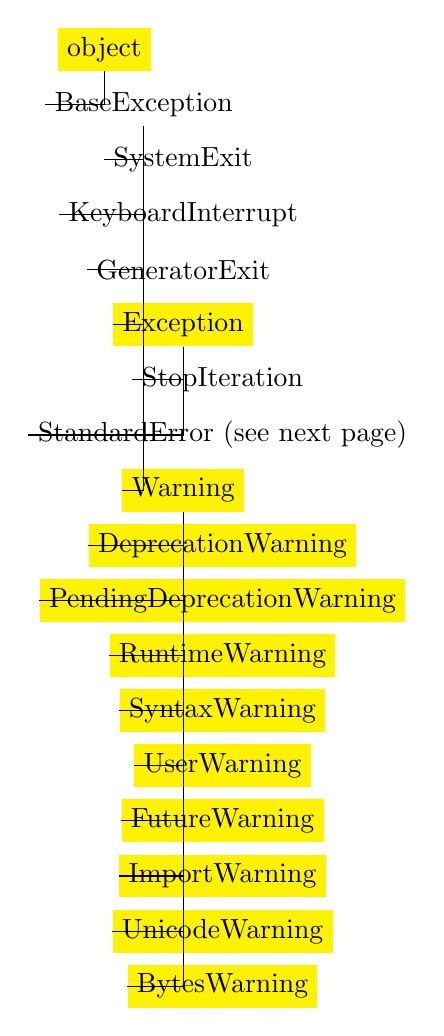
\begin{tikzpicture}[%
    grow via three points={one child at (0.5,-0.7) and
    two children at (0.5,-0.7) and (0.5,-1.4)},
    edge from parent path={(\tikzparentnode.south) |- (\tikzchildnode.west)}]
    \node [fill=yellow] {object}
    child { node {BaseException}
      child { node {SystemExit}}
      child { node {KeyboardInterrupt}}
      child { node {GeneratorExit}}
      child { node [fill=yellow] {Exception}
        child {node {StopIteration}}
        child {node {StandardError (see next page)}}
      }
      child [missing] {}
      child [missing] {}
      child { node [fill=yellow] {Warning}
        child { node [fill=yellow] {DeprecationWarning}}
        child { node [fill=yellow] {PendingDeprecationWarning}}
        child { node [fill=yellow] {RuntimeWarning}}
        child { node [fill=yellow] {SyntaxWarning}}
        child { node [fill=yellow] {UserWarning}}
        child { node [fill=yellow] {FutureWarning}}
        child { node [fill=yellow] {ImportWarning}}
        child { node [fill=yellow] {UnicodeWarning}}
        child { node [fill=yellow] {BytesWarning}}
      }
    };
\end{tikzpicture}
\vskip.1cm
All instances of exceptions can have \verb|tostring(e)| and \verb|repr(e)| called on them, both of which will return the message that was passed to the exception.
Users should extend the \verb|Exception| class when creating their own exceptions as shown below:
\begin{verbatim}
class MyException extends Exception:
    def MyException(message : string):
        Exception.Exception(message)
\end{verbatim}

\pagebreak
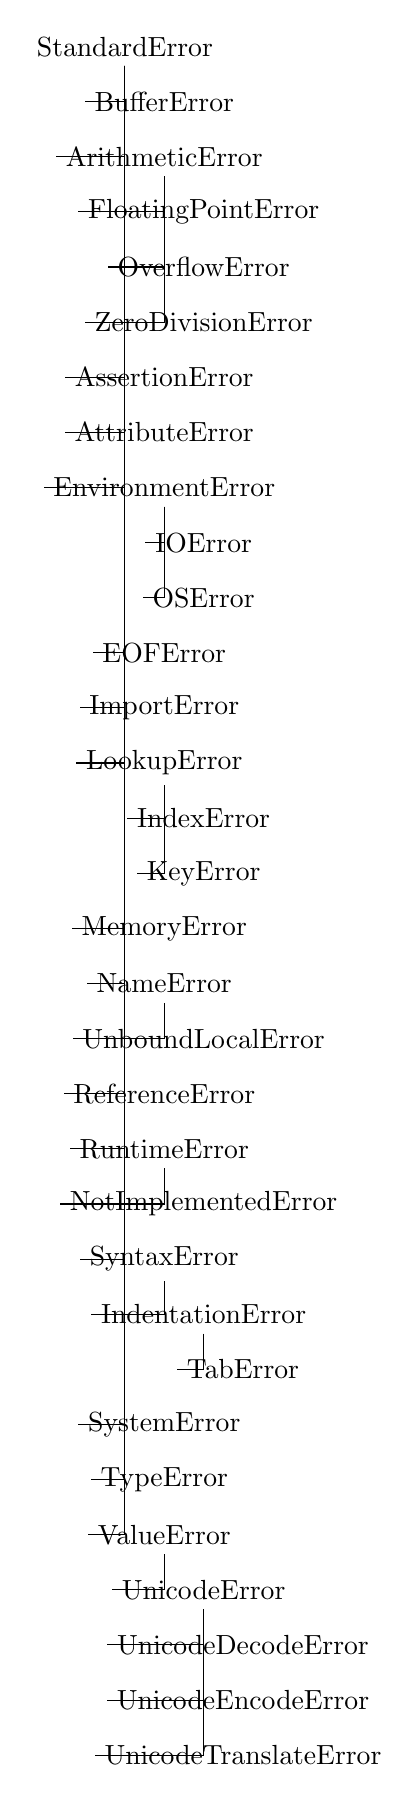
\begin{tikzpicture}[%
    grow via three points={one child at (0.5,-0.7) and
    two children at (0.5,-0.7) and (0.5,-1.4)},
    edge from parent path={(\tikzparentnode.south) |- (\tikzchildnode.west)}]
    \node {StandardError}
        child { node {BufferError}}
        child { node {ArithmeticError}
            child { node {FloatingPointError}}
            child { node {OverflowError}}
            child { node {ZeroDivisionError}}
        }
        child [missing] {}
        child [missing] {}
        child [missing] {}
        child { node {AssertionError}}
        child { node {AttributeError}}
        child { node {EnvironmentError}
            child { node {IOError}}
            child { node {OSError}}
        }
        child [missing] {}
        child [missing] {}
        child { node {EOFError}}
        child { node {ImportError}}
        child { node {LookupError}
            child { node {IndexError}}
            child { node {KeyError}}
        }
        child [missing] {}
        child [missing] {}
        child { node {MemoryError}}
        child { node {NameError}
            child { node {UnboundLocalError}}
        }
        child [missing] {}
        child { node {ReferenceError}}
        child { node {RuntimeError}
            child { node {NotImplementedError}}
        }
        child [missing] {}
        child { node {SyntaxError}
            child { node {IndentationError}
                child { node {TabError}}
            }
        }
        child [missing] {}
        child [missing] {}
        child { node {SystemError}}
        child { node {TypeError}}
        child { node {ValueError}
            child { node {UnicodeError}
                child { node {UnicodeDecodeError}}
                child { node {UnicodeEncodeError}}
                child { node {UnicodeTranslateError}}
            }
        }
        ;
\end{tikzpicture}

\pagebreak

\section{CSPy Graphics Library}
\subsection{The Basics}
To import the library, the line "\verb|from cs110graphics pyimport *|" needs to be the first line of your program. To put objects into the Graphics System, it requires a function which takes an object of type Window as a parameter.
\begin{verbatim}
    def function(win:Window):
\end{verbatim}
There are seven types of objects you can add to a window. Text, Image, Oval, Circle, Rectangle, Square, and Polygon. Each has its own method of initalization and requires specific parameters, but like the above function, each function requires a window object as the first parameter.

\begin{verbatim}
    def function(win:Window):
        ::circ:Circle::
        circ = Circle(win, 40, (200, 200))
        win.add(circ)
\end{verbatim}

To start the graphics system, instead of initalizing a function by calling it, you would wrap the function in a function called \verb|StartGraphicsSystem|. 
\begin{verbatim}
    def function(win:Window):
        ::circ:Circle::
        circ = Circle(win, 40, (200, 200))
        win.add(circ)

    StartGraphicsSystem(function)
\end{verbatim}

\begin{figure}[h!]

\includegraphics[width=.5\textwidth]{circle}
\centering
\captionof{figure}{The above code yields a circle of radius 40 in the center of the window.}
\end{figure}

The next page contains all of the graphical objects which are included in the graphics library, as well as sample code and implementations.

\pagebreak
\begin{itemize}
\item Text requires a string of text, but can optionally take a font size and a center. 
\begin{figure}[h!]
\centering
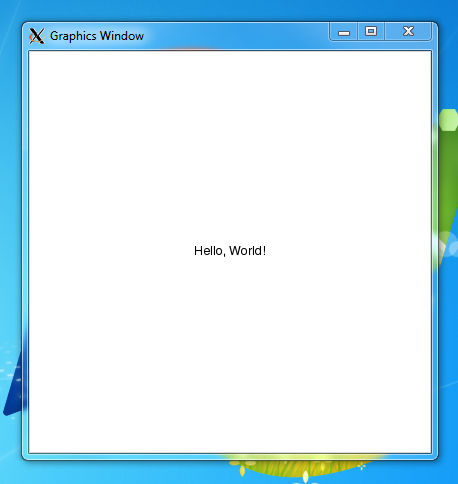
\includegraphics[width=.5\textwidth]{text}
\captionof{figure}{Text(win, "Hello, World!", 12, (200, 200))}
\end{figure}

\item Image requires a name of an image, which has to be in the current working directory. It can optionally take a width, a height, and a center. 
\begin{figure}[h!]
\centering
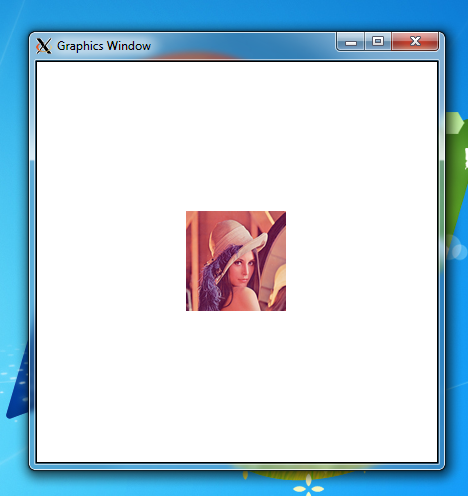
\includegraphics[width=.5\textwidth]{image}
\captionof{figure}{Image(win, "Lenna.png", 100, 100, (200, 200))}
\end{figure}

\pagebreak
\item Circles require a window, but can optionally take a radius and a center. 
\begin{figure}[h!]
\centering

\includegraphics[width=.5\textwidth]{circle}
\captionof{figure}{Circle(win, 40, (200, 200))}
\end{figure}

\item Ovals require a window, but can optionally take a radiusX, a radiusY, and a center. 
\begin{figure}[h!]
\centering
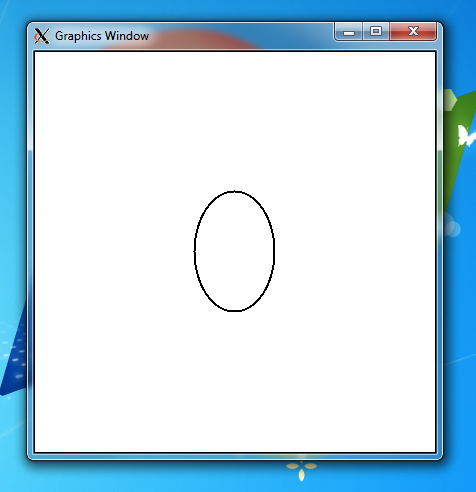
\includegraphics[width=.5\textwidth]{oval}
\captionof{figure}{Oval(win, 40, 60, (200, 200))} 
\end{figure}

\pagebreak

\item Squares require a window, but can optionally take a side length and a center. 
\begin{figure}[h!]
\centering
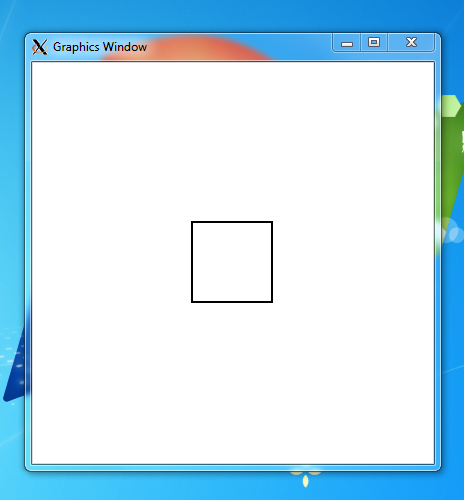
\includegraphics[width=.5\textwidth]{square}
\captionof{figure}{Square(win, 40, (200, 200))}
\end{figure}

\item Rectangles require a window, but can optionally take a width, a height, and a center. 
\begin{figure}[h!]
\centering
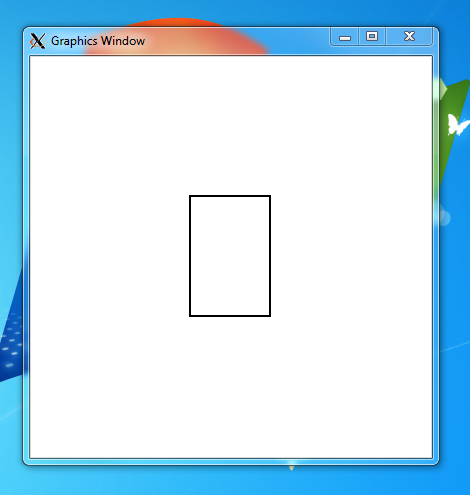
\includegraphics[width=.5\textwidth]{rectangle}
\captionof{figure}{Rectangle(win, 40, 60, (200, 200))}
\end{figure}

\pagebreak
\item Polygons require a window and a list of points. It cannot take anything optionally. 
\begin{figure}[h!]
\centering
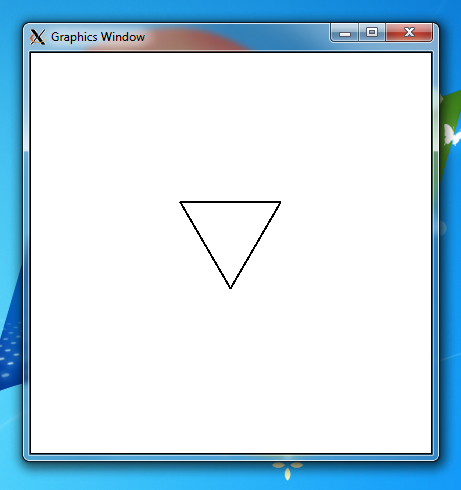
\includegraphics[width=.5\textwidth]{polygon}
\captionof{figure}{Polygon(win, [(150, 150), (200, 236), (250, 150)])}
\end{figure}
\end{itemize}

\subsection{More Specific Methods}
Objects of type \verb|GraphicalObject| have access to \verb|GraphicalObject| methods, and Objects of type \verb|Fillable| have access to \verb|Fillable| methods, as well as \verb|GraphicalObject| methods. Some classes even have their own methods which can be accessed only by them.
\vskip.2in
\verb|GraphicalObjects| are all seven types of object that can be put on the canvas. They have the following methods accessible:

\begin{itemize}
\item \verb|add_handler(graphic:GraphicalObject)| - initalizes an EventHandler on the object and allows for overwriting of EventHandler functions by the class. (See Event Handling later in this section.)
\item \verb|get_center() -> tuple of (int * int)| - returns the center of the \verb|GraphicalObject|.
\item \verb|get_depth() -> int| - returns the depth of the \verb|GraphicalObject|.
\item \verb|move(dx:int, dy:int)| - Moves a \verb|GraphicalObject| dx pixels horizontally and dy pixels vertically.
\item \verb|move_to(point:tuple of (int * int))| - moves the center of a \verb|GraphicalObject| to the point.
\item \verb|set_depth(depth:int)| - sets the depth of the \verb|GraphicalObject|.
\end{itemize}
\vskip.2in
\verb|Fillables| are five of the objects that can be put on the canvas. They can have their fill colors and border colors changed, among other things. The \verb|Circle|, \verb|Oval|, \verb|Rectangle|, \verb|Square|, and \verb|Polygon| objects are all \verb|Fillables|.

\begin{itemize}
\item \verb|get_border_color() -> string| - returns the border color of a Fillable.
\item \verb|get_border_width() -> int| - returns the border width of a Fillable.
\item \verb|get_fill_color() -> string| - returns the fill color of a Fillable.
\item \verb|get_pivot() -> tuple of (int * int)| - returns the pivot point of a Fillable.
\item \verb|rotate(degrees:int)| - rotates a Fillable by degrees.
\item \verb|scale(factor:float)| - scales a Fillable's size by the scale factor. 
\item \verb|set_border_color(color:string)| - sets the border color of the Fillable.
\item \verb|set_border_width(width:int)| - sets the border width of the Fillable.
\item \verb|set_fill_color(color:string)| - sets the fill color of the Fillable.
\item \verb|set_pivot(pivot:tuple of (int * int))| - sets the pivot point of the Fillable.
\end{itemize}
You can either use names of colors like "\verb|yellow|", or you can use hexadecimal numbers in a string like "\verb|#FFFF00|" to set a color.

\begin{figure}[h]
\centering
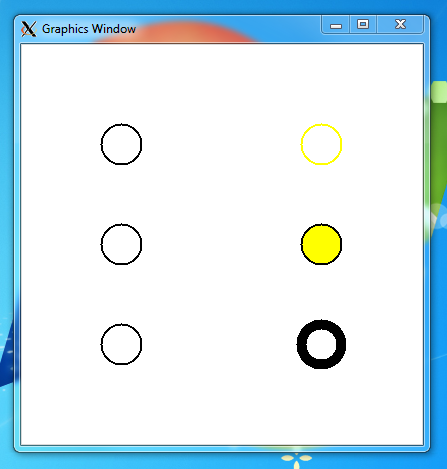
\includegraphics[width=.5\textwidth]{fillableAttributes}
\captionof{figure}{circ.set\_border\_color("yellow"), circ.set\_fill\_color("yellow"), circ.set\_border\_width(10)}

\end{figure}

Image methods (not including any inherited methods from GraphicalObject):
\begin{itemize}
\item \verb|resize(width:int, height:int)| - resizes an Image by width and height.
\item \verb|rotate(degrees:int)| - rotates an Image by degrees.
\item \verb|scale(factor:float)| - scales an Image's size by scale factor
\item \verb|size() -> tuple of (int * int)| - returns a tuple of the width and height of an Image.

\begin{figure}[h]
\centering
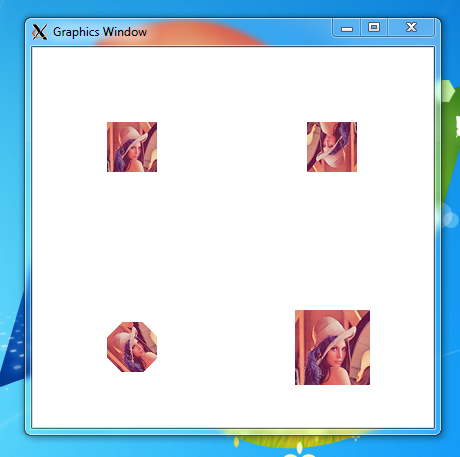
\includegraphics[width=.5\textwidth]{imageAttributes}
\captionof{figure}{img.rotate(180), img.rotate(45), img.scale(1.5)}
\end{figure}

\pagebreak

\end{itemize}
Text methods (not including any inherited methods from GraphicalObject):
\begin{itemize}
\item \verb|set_text(text:string)| - Sets the text of the Text object.
\item \verb|set_size(size:int)| - sets the point size of the Text object.
\end{itemize}
\vskip.1in
Circle methods (not including any inherited methods from GraphicalObject or Fillable):
\begin{itemize}
\item \verb|set_radius(radius:int)| - sets the radius of the Circle.
\end{itemize}
\vskip.1in
Oval methods (not including any inherited methods from GraphicalObject or Fillable):
\begin{itemize}
\item \verb|set_radii(radiusX:int, radiusY:int)| - sets the radii of the Oval.
\end{itemize}
\vskip.1in
Square methods (not including any inherited methods from GraphicalObject or Fillable):
\begin{itemize}
\item \verb|set_side_length(sideLength:int)| - sets the side length of the Square.
\end{itemize}
\vskip.1in
Rectangle methods (not including any inherited methods from GraphicalObject or Fillable):
\begin{itemize}
\item \verb|set_side_lengths(width:int, height:int)| - sets the width and height of the Rectangle. 
\end{itemize}

\subsection{Event Handling}
Event handling is the computer science term for sending keyboard and mouse commands to a graphical interface. The graphics library supports a rudimentary version of event handling.

There are two classes which do the work: \verb|Event|, and \verb|EventHandler|. \verb|Event| takes an keyboard or mouse event and converts it to a format which can be read by \verb|EventHandler|. In \verb|Event|, you can get the location where the event occurred, the mouse button that did it, the keyboard button that did it, or a description of the event. This is useful for handling different kinds of button input.
\vskip.1in
Below is a list of Event's methods:

\begin{itemize}
\item \verb|get_button() -> string| - returns the mouse button that generated the event. It will be one of the following:
\begin{itemize}
\item Left Mouse Button
\item Middle Mouse Button
\item Right Mouse Button
\end{itemize}
\item \verb|get_description() -> string| - returns the description of the event. It will be one of the following:
\begin{itemize}
\item Key Press
\item Key Release
\item Mouse Press
\item Mouse Release
\item Mouse Move
\item Mouse Enter
\item Mouse Leave
\end{itemize}
\item \verb|get_key() -> string| - returns the key that was pressed or released.
\item \verb|get_location() -> tuple of (int * int)| - returns the location of the mouse on the canvas.
\item \verb|get_root_location() -> tuple of (int * int)| - returns the location of the mouse on the monitor.
\end{itemize}

\verb|EventHandler| is a class which contains what is executed when an event is sent to specific objects. It is designed so that the user can overwrite the functions in the class and replace it with their own functions.
\vskip.1in
The functions that can be overwritten are as follows:
\begin{itemize}
\item \verb|handle_key_press(event:Event)| - handles a key press. 
\item \verb|handle_key_release(event:Event)| - handles a key release. 
\item \verb|handle_mouse_enter(event:Event)| - handles when the mouse enters an object. 
\item \verb|handle_mouse_leave(event:Event)| - handles when the mouse leaves an object. 
\item \verb|handle_mouse_move(event:Event)| - handles mouse movement. 
\item \verb|handle_mouse_press(event:Event)| - handles a mouse press. 
\item \verb|handle_mouse_release(event:Event)| - handles a mouse release. 
\end{itemize}

To overwrite, the user has to extend EventHandler and initalize it in their custom class:

\begin{verbatim}
class Button extends EventHandler:
    :: circ:Circle::
    def Button(win:Window):
        EventHandler.EventHandler()
        circ = Circle(win)
        win.add(circ)
        circ.add_handler(self)
\end{verbatim}

The user has defined a class called Button, which takes no parameters. The EventHandler is initalized, the Button's representation is made, and then the Button gets the ability to overload functions in EventHandler using the \verb|add_handler()| function.

To overwrite a function, all you have to do is define a function that matches the names of the functions you want to overwrite. If for example, the user wants the circle's color to change when they click on it, they would do this:

\begin{verbatim}
def handle_mouse_release(event:Event):
    circ.set_fill_color("yellow")
\end{verbatim}

After that is written by the user and run, the object's fill color will turn yellow when it is clicked. 

Each function requires an object of type Event to be attached so that if the user wants to know more details about the EventHandler, they can access the Event methods discussed above. For example, what if the user wants to know where the mouse was clicked within an object? The user would then use the Event class and call getMouseLocation() to find out:

\begin{verbatim}
def handle_mouse_release(event:Event):
    print(event.get_mouse_location())
\end{verbatim}

\subsection{Animations}

There are two ways to do animations. One is to use the Timer class. When initalized, a Timer takes a window, a delay (in milliseconds), and a function. The timer will re-run the function after each delay of time. To start the timer, call the \verb|start()| function. To stop the timer, call the \verb|stop()| function.

\begin{verbatim}
class Button:
    :: circ:Circle, timer:Timer, pressed:bool ::
    def Button(win:Window):
        circ = Circle(win)
        win.add(circ)
        timer = Timer(win, 200, flash)
        pressed = False
        timer.start()

    def flash():
        if pressed:
            circ.set_fill_color("")
            pressed = False
        else:
            circ.set_fill_color("yellow")
            pressed = True
\end{verbatim}

This code example has several parts to it. It first initalizes a Circle, a Timer and a Boolean. It creates the circle, adds it, creates the timer, sets the boolean to False, then starts the timer. The timer then runs the function \verb|flash|, which sets the fill color to yellow, then after 200 seconds sets it to be transparent.

Another way to do animations is to run an instance of the \verb|RunWithYieldDelay| class. This class takes a function which has the CSPy keyword \verb|yield| and then allows that function to run with a delay.

\begin{verbatim}
def main(win:Window):
    :: circ:Circle ::
    circ = Circle(win)
    win.add(circ)
    RunWithYieldDelay(win, move_circle(circ))

def move_circle(circ:Circle) -> generator of int:
    for i in range(10):
        circ.move(10, 0)
        yield 200
    raise StopIteration
\end{verbatim}

This function will keep running until the for loop stops.

\pagebreak

\section{Appendix 1: Types}
\textbf{Int:} A numeric type.\\
Binary Operators:\\
\begin{tabular}{|c|c|}
\hline
Addition & \verb|+| \\
\hline
Subtraction & \verb|-| \\
\hline
Multiplication & \verb|*| \\
\hline
Division & \verb|/| \\
\hline
Floor Division & \verb|//| \\
\hline
Exponentiation & \verb|**| \\
\hline
Modulus & \verb|%| \\
\hline
Bitwise And & \verb|&| \\
\hline
Bitwise Or & \verb!|! \\
\hline
Bitwise Xor & \verb|^| \\
\hline
Bitwise Invert & \verb|~| \\
\hline
Equals & \verb|==| \\
\hline
Not Equals & \verb|!=| \\
\hline
Greater Than & \verb|>| \\
\hline
Less Than & \verb|<| \\
\hline
Greater Or Equal To & \verb|>=| \\
\hline
Less Or Equal To & \verb|<=| \\ 
\hline
Bitwise Left Shift & \verb|<<| \\
\hline
Bitwise Right Shift & \verb|>>| \\
\hline
\end{tabular}
\vskip.2in
Unary Operators:\\
\begin{tabular}{|c|c|}
\hline
Positive & + \\
\hline
Negative & - \\
\hline
\end{tabular}
\vskip.2in
Type Conversion:
\begin{itemize}
\item Float via the \verb|tofloat| built in function
\item String via the \verb|tostring| or \verb|repr| built in function
\end{itemize}
Additional Operations:
\begin{itemize}
\item Supports augmented assignment.
\end{itemize}
\vskip.2in

\textbf{Float:} A numeric type.
\vskip.1in
Binary Operators: \\
\begin{tabular}{|c|c|}
\hline
Addition & \verb|+| \\
\hline
Subtraction & \verb|-| \\
\hline
Multiplication & \verb|*| \\
\hline
Division & \verb|/| \\
\hline
Floor Division & \verb|//| \\
\hline
Exponentiation & \verb|**| \\
\hline
Modulus & \verb|%| \\
\hline
Equals & \verb|==| \\
\hline
Not Equals & \verb|!=| \\
\hline
Greater Than & \verb|>| \\
\hline
Less Than & \verb|<| \\
\hline
Greater Or Equal To & \verb|>=| \\
\hline
Less Or Equal To & \verb|<=| \\ 
\hline
\end{tabular}
\vskip.2in
Unary Operators:\\
\begin{tabular}{|c|c|}
\hline
Positive & + \\
\hline
Negative & - \\
\hline
\end{tabular}
\vskip.2in
Type Conversion:
\begin{itemize}
\item Int via the \verb|toint| or \verb|round| built in function
\item String via the \verb|tostring| or \verb|repr| built in function
\end{itemize}
Additional Operations:
\begin{itemize}
\item Supports augmented assignment.
\end{itemize}
\vskip.2in

\textbf{Bool:} \\
Binary Operators: \\
\begin{tabular}{|c|c|}
\hline
Boolean And & \verb|and| \\
\hline
Boolean And & \verb|&&| \\
\hline
Boolean Or & \verb|or| \\
\hline
Boolean Or & \verb!||! \\
\hline
\end{tabular}
\vskip.2in
Unary Operators:\\
\begin{tabular}{|c|c|}
\hline
Boolean Not & \verb|not| \\
\hline
\end{tabular}
\vskip.2in
Type Conversion:
\begin{itemize}
\item String via the \verb|tostring| or \verb|repr| built in function
\end{itemize}
(NOTE: In Python, bool is a subclass of Integer, therefore Integer binary operators such as '+', '-', etc. would be applicable to Boolean values as well. This is not the case in CSPy, as there is no benefit for a beginner programmer to use any of these operators on boolean.) \\
\vskip.2in
\textbf{String:} A sequence type.
\vskip.1in
Binary Operators: \\
\begin{tabular}{|c|c|}
\hline
Concatenate & \verb|+| \\
\hline
Repetition & \verb|*| \\
\hline
Greater Than & \verb|>| \\
\hline
Less Than & \verb|<| \\
\hline
Greater Or Equal To & \verb|>=| \\
\hline
Less Or Equal To & \verb|<=| \\ 
\hline
Equals & \verb|==| \\
\hline
Not Equals & \verb|!=| \\ 
\hline
\end{tabular}
\vskip.2in
Type Conversion:
\begin{itemize}
\item Integer via \verb|toint| built-in function 
\item Float via \verb|tofloat| built-in function
\item List, Set, or Frozenset via \verb|tolist| or \verb|makeset| or \verb|frzset| built-in functions
\end{itemize}
Additional Operations:
\begin{itemize}
\item String supports indexing, slicing, membership, iterations, and use of the \verb|len()| function. Also supports augmented assignment. 
\end{itemize}

\vskip.2in
\textbf{List:} A sequence type.
\vskip.1in
Binary Operators: \\
\begin{tabular}{|c|c|}
\hline
Concatenate & \verb|+| \\
\hline
Repetition & \verb|*| \\
\hline
Equals & \verb|==| \\
\hline
Not Equals & \verb|!=| \\ 
\hline
\end{tabular}
\vskip.2in
Type Conversion:
\begin{itemize}
\item String via \verb|tostring| or \verb|repr| built-in function
\item Set or Frozenset via \verb|makeset| or \verb|frzset| built-in functions
\item Bool via \verb|tobool| built-in function
\end{itemize}
Additional Operations:
\begin{itemize}
\item List supports indexing, slicing, membership, iterations, and use of the \verb|len()| function. Also supports augmented assignment. 
\end{itemize}
\vskip.2in

\textbf{Tuples:} A sequence type.
Tuples are heterogeneous, and can contain elements of multiple types. Tuples are also immutable and can't be changed once created.
\vskip.1in
Binary Operators: \\
\begin{tabular}{|c|c|}
\hline
Concatenate & \verb|+| \\
\hline
Repetition & \verb|*| \\
\hline
Equals & \verb|==| \\
\hline
Not Equals & \verb|!=| \\ 
\hline
\end{tabular}
\vskip.2in
Type Conversion:
\begin{itemize}
\item String via \verb|tostring| or \verb|repr| built-in function
\item List, Set or Frozenset via \verb|tolist|, \verb|makeset| or \verb|frzset| built-in functions (only applicable for homogeneous tuples)
\end{itemize}
Additional Operations:
\begin{itemize}
\item Tuples support indexing, slicing, membership testing, iteration, and use of the \verb|len()| function. Tuples do not support augmented assignment (they are immutable). 
\end{itemize}
(NOTE: The methods for tuples have generic “object” return types because the return type of these operators depends on the type of the tuple. Since tuples can contain multiple types unlike lists, the return type of a slicing or indexing operation is determined in the type checker by analyzing the elem\_type list of the tuple. Because it is impossible to determine the return type of an indexing or slicing operation of a multi-typed tuple using a variable as an index, indexing tuples with variables is NOT allowed. 
\begin{center}
\verb|mytuple[2]| \verb|->| acceptable \\
\verb|mytuple[p]| \verb|->| unacceptable
\end{center}
Similarly, because it is impossible to determine the type of an iterative variable in a for loop iterating over a multi-type tuple, tuples DO NOT support iterating.) 
\vskip.2in

\textbf{Dictionary:} An associative array.
\vskip.1in
Binary Operators: \\
\begin{tabular}{|c|c|}
\hline
Equals & \verb|==| \\
\hline
Not Equals & \verb|!=| \\ 
\hline
\end{tabular}
\vskip.2in
Type Conversion:
\begin{itemize}
\item String via \verb|tostring| or \verb|repr| built-in function
\item List, Set or Frozenset via \verb|tolist|, \verb|makeset| or \verb|frzset| built-in functions
\item Bool via \verb|tobool| built-in function
\end{itemize}
Additional Operations:
\begin{itemize}
\item Dictionaries support indexing, slicing, membership testing, iteration, and use of the len() function. 
\end{itemize}
\vskip.2in

\textbf{Sets and Frozensets:} \\ 
An unordered collection of unique elements. Sets  and frozensets are homogeneous, i.e. they can only contain one element type. Sets are mutable but frozensets are immutable. 
\vskip.1in
Binary Operators: \\
\begin{tabular}{|c|c|}
\hline
Proper Subset & \verb|<| \\
\hline
Proper Superset & \verb|>| \\
\hline
Superset & \verb|<=| \\
\hline
Superset & \verb|>=| \\
\hline
Union & \verb!|! \\
\hline
Intersection & \verb|&| \\
\hline
Difference & \verb|-| \\
\hline
Symmetric Difference & \verb|^| \\
\hline
Not Equal & \verb|!=| \\
\hline
Equals & \verb|==| \\
\hline
\end{tabular}
\vskip.2in
Type Conversion:
\begin{itemize}
\item String via \verb|tostring| or \verb|repr| built-in function
\item List, Set or Frozenset via \verb|tolist|, \verb|makeset| or \verb|frzset| built-in functions
\item Bool via \verb|tobool| built-in function
\end{itemize}
Additional Operations:
\begin{itemize}
\item Sets and frozensets support membership testing and iteration. Sets support augmented assignment. Frozensets do not (they are immutable). 
\end{itemize}
\vskip.2in
\textbf{Functions:} \\
A function is a procedure that returns a value. Functions have a return type. All of the return statements in a function must be nonempty and their return value must have the same type as the function’s return type.

CSPy supports function overloading, provided that each function or procedure has a distinct parameter list. (NOTE: See CSPy Grammar Rules - Functions and Procedures for more details.)

A declared variable may be bound to a function:
\begin{verbatim}
    f:fn (int, int) -> int = add
\end{verbatim}
The above will assign the overloaded add function corresponding to the given type signature to f. Similarly, the below example is also valid because the type of the anonymous function matches the type of f:
\begin{verbatim}
    f:fn (int, int) -> int = lambda (x:int, y:int) -> int : (x + y)
\end{verbatim}
(NOTE: \verb|fn (int, ?int) -> int| is not equivalent to \verb|fn (int, int) -> int|. The \verb|?| symbol in the first function type indicates the second integer is an optional parameter.  This is the same for procedures.)
\vskip.2in

\textbf{Procedures:} \\
A procedure does not return a value and hence has no return type. Procedures support function overloading as well. (NOTE: See CSPy Grammar Rules - Functions and Procedures for more details.)

Declared variables may be bound to procedures using the following syntax:
\begin{verbatim}
    p:proc (int) = output
\end{verbatim}
\vskip.2in

\textbf{Files:} \\
Files are the type for a Python file object. A file is created by using the built-in open() function. Attributes of the file type are as follows:
\begin{itemize}
\item \verb|closed:bool| - True if the file is closed, False otherwise.
\item \verb|name:string| - The name of the file.
\item \verb|mode:string| - The mode which the file was opened with.
\end{itemize}

\pagebreak

\section{Appendix 2: Built In Functions}

\textbf{Python Built Ins:}
(NOTE: Not all of the built-in Python functions are implemented in CSPy. The below functions have been implemented.)
\begin{itemize}
\item \verb|abs(x:int) -> int| \\
      \verb|abs(x:float) -> float| \\
  Returns the absolute value of x.

\item \verb|all(l:list of ?) -> bool| \\
  Returns true if all the elements in l are true.

\item \verb|any(l:list of ?) -> bool| \\
  Returns true if any of the elements in l are true. 

\item \verb|bin(x:int) -> string| \\
 Converts x into a binary string. 

\item \verb|chr(i:int) -> string| \\
   Returns a string representing a character whose Unicode point is i.

\item \verb|cmp(a:int, b:int) -> int| \\
\verb|cmp(a:float, b:float) -> int| \\
\verb|cmp(a:string, b:string) -> int| \\
\verb|cmp(a:bool, b:bool) -> int| \\
\verb|cmp(a:list, b:list) -> int| \\
\verb|cmp(a:tuple, b:tuple) -> int| \\
\verb|cmp(a:dict, b:dict) -> int| \\
\verb|cmp(a:set, b:set) -> int| \\
\verb|cmp(a:frozenset, b:frozenset) -> int| \\
Returns 1 if a $>$ b, -1 if a $<$ b, and 0 if a == b. 

\item \verb|divmod(a:int, b:int) -> tuple of (int * int)| \\
 \verb|divmod(a:float, b:float) -> tuple of (float * float)| \\
Returns a pair of numbers consisting of the quotient of a and b and their remainder when using integer division. For integers, this is equivalent to \verb|(a // b, a % b)|. For floats, this is equivalent to \verb|(math.floor(a / b), a % b)|. 

\item \verb|exit(?code:int)| \\
    Exits from the current program. 

\item \verb|hex(x:int) -> string| \\
Converts x to a lowercase hexadecimal string prefixed with '0x'.

\item \verb|len(s:string) -> int|
\verb|len(l:list) -> int| \\
\verb|len(t:tuple) -> int| \\
\verb|len(d:dict) -> int| \\
\verb|len(mset:set) -> int| \\
\verb|len(fr:frozenset) -> int| \\
Returns the number of objects in the given sequence or container. 

\item \verb|max(a:int, b:int) -> int|
\verb|max(a:float, b:float) -> float| \\
\verb|max(l:list of elem_type) -> elem_type| \\
For integers and floats, returns a if a $>$ b or b if b $>$ a. For lists, returns the item from the list with max value. 

\item \verb|map(f:func, l:list) -> list|
\verb|map(f:func, d:dict) -> dict| \\
\verb|map(f:func, t:tuple) -> tuple| \\
\verb|map(f:func, mset:set) -> set| \\
\verb|map(f:func, fr:frozenset) -> frozenset| \\
Applies the function f to each value within the given sequence or container and returns a new container.

\item \verb|min(a:int, b:int) -> int|
\verb|min(a:float, b:float) -> float| \\
\verb|min(l:list of elem_type) -> elem\_type| \\
For integers and floats, returns a if a $<$ b or b if b $<$ a. For lists, returns the item from the list with min value. 

\item \verb|oct(x:int) -> string| \\
 Converts x to an octal string. 

\item \verb|ord(s:string) -> int| \\
 Given a string representing a Unicode character s, returns an integer
 representing the Unicode point of s.

\item \verb|open(name:string, mode:string = "r") -> file| \\
Open the file name in mode. If mode is not given, defaults to “r” (read). Returns a file object. 

\item \verb|print(output:string)| \\
Prints the ouput string to the console with a newline at the end.

\item \verb|pow(x:int, y:int) -> int| \\
\verb|pow(x:int, y:int, z:int) -> int| \\
Returns x to the power y. If z is present, returns x to the power y 
modulo z.

\item \verb|range(stop:int) -> list of int| \\
\verb|range(start:int, stop:int, step:int = 1 ) - > list of int| \\
Returns a list of integers representing the range of integers from start to stop using step if given. If only stop is given, start defaults to 0.  

\item \verb|round(x:float, y:int = 0) -> int| \\
Returns x rounded to y digits after the decimal point. If y is omitted, returns the nearest integer to its input. 

\item \verb|sum(l:list of int, start:int = 0) -> int| \\
\verb|sum(l:list of float, start:float = 0.0) -> float| \\
\verb|sum(t:tuple of int, start:int = 0) -> int| \\
\verb|sum(t:tuple of float, start:float = 0.0) -> float| \\
\verb|sum(t:set of int, start:int = 0) -> int| \\
\verb|sum(t:set of float, start:float = 0.0) -> float| \\
\verb|sum(t:frozenset of int, start:int = 0) -> int| \\
\verb|sum(t:frozenset of float, start:float = 0.0) -> float| \\
Sums start and the items of the iterable from left to right and returns the total. start defaults to 0 if not given. 
\end{itemize}
\vskip.2in

\textbf{String Built Ins:}
\begin{itemize}
\item \verb|capitalize() -> string| \\
    Capitalizes a string. 

\item \verb|center(width:int, ?fillchar:string = “ “) -> string| \\
Returns a centered string of length width whose padding is done using the specified fill character. The default fill character is a space. 

\item \verb|count(str:string, ?beg:int = 0, ?end: int = len(string)) -> int| \\
Counts how many times str occurs in string or in a substring of the current string if the starting index beg and ending index end are given. 

\item \verb|decode(?encoding = “UTF-8”, ?errors = “strict”) -> string| \\
Decodes the current string using the codec encoding, which defaults to the default string encoding. Errors is the error handling scheme, which defaults to “strict”, meaning encoding errors will raise a UnicodeError. 

\item \verb|encode(?encoding = “UTF-8”, ?errors = “strict”) -> string| \\
Encodes the current string using the codec encoding, which defaults to the default string encoding. Errors if the error handling scheme, which defaults to “strict”, meaning encoding errors will raise a UnicodeError. 

\item \verb|endswith(suffix:string, ?beg:int = 0, ?end:int = len(string)) -> bool| \\
Determines whether or not the current string ends with suffix (or a substring of a string if starting index beg and ending index end are given). 

\item \verb|expandtabs(?tabsize:int = 8) -> string| \\
Expands tabs in string to multiple spaces. Defaults to 8 spaces per tab if tabsize is not provided. 

\item \verb|find(str:string, ?beg:int = 0, ?end:int = len(string)) -> int| \\
Determines if str occurs in the current string or in a substring if starting index beg and ending index end are given. Returns starting index of str if found, else returns -1. 

\item \verb|index(str:string, ?beg:int = 0, ?end:int = len(string)) -> int| \\
    Same as find, but raises an exception is str is not found. 

\item \verb|isalnum() -> bool| \\
Returns true if string has at least 1 character and all the characters are alphanumeric. 

\item \verb|isalpha() -> bool| \\
    Same as isalnum. 

\item \verb|isdigit() -> bool| \\
    Returns true if the string contains only digits.

\item \verb|islower() -> bool| \\
Returns true if string has at least 1 cased character and all cased characters are in lowercase. 

\item \verb|isnumeric() -> bool| \\
    Returns true if a Unicode string contains only numeric characters. 

\item \verb|isspace() -> bool| \\
    Returns true if the string contains only whitespace characters. 

\item \verb|istitle() -> bool| \\
    Returns true if the string is properly “titlecased”. 

\item \verb|isupper() -> bool| \\
Returns true if string has at least one cased character and all cased characters are in uppercase. 

\item \verb|join(seq:list/tuple of string) -> string| \\
Concatenates the elements in the sequence into a string with the current string as a separator. The elements in the sequence must be strings. 

\item \verb|ljust(width:int, ?fillchar:string = “ “) -> string| \\
Returns a left justified string of length width whose padding is fillchar, which defaults to a space. 

\item \verb|lower() -> string| \\
    Converts all uppercase letters to lowercase. 

\item \verb|lstrip() -> string| \\
    Removes all leading whitespace in the current string. 

\item \verb|replace(old:string, new:string, max:int) -> string| \\
Returns a copy of the string with all occurrences of the substring old replaced by new if max is not specified. If max is specified, only max occurrences will be replaced starting from the front of the string. 

\item \verb|rfind(str:string, ?beg:int = 0, ?end:int = len(string)) -> int| \\
    Same as find(), but searches backwards in the string.

\item \verb|rindex(str:string, ?beg:int = 0, ?end:int = len(string)) -> int| \\
    Same as index(), but searches backwards in the string. 

\item \verb|rjust(width:int, ?fillchar:string = “ “) -> string| \\
Returns the original string right justified to a total width of columns using fillchar, which defaults to a space. 

\item \verb|rstrip() -> string| \\
    Removes all of the trailing whitespace on a string. 

\item \verb|split(str:string = “ ”,  ?num:int = string.count(str)) -> list of string| \\
Splits strings according to str (defaults to a space) and returns a list of substrings. Splits into at most num substrings if num is given. 

\item \verb|splitlines(?num:int = string.count(”\n”)) -> list of string| \\
Splits at all (or num if given) new lines and returns a list of each line with newlines removed. 

\item \verb|startswith(str:string, ?beg:int = 0, ?end:int = len(string)) -> bool| \\
Determines if the current string (or a substring of string if the starting index beg and ending index end are given) starts with the substring str. 

\item \verb|strip() -> string| \\
    Performs both lstrip() and rstrip() at the same time. 

\item \verb|swapcase() -> string| \\
    Inverts the case for all letters in a string. 

\item \verb|title() -> string| \\
Returns “titlecased” version of the current string where all words begin with uppercase letters and the rest are lowercase. 

\item \verb|upper() -> string| \\
    Converts lowercase letters in the current string to uppercase. 
\end{itemize}
\vskip.2in

\textbf{List Built Ins:}
\begin{itemize}
\item \verb|append(obj:elem_type)| \\
    Appends obj to the end of the list. 

\item \verb|count(obj:elem_type) -> int| \\
    Returns count of how many times obj occurs in list.

\item \verb|extend(seq:list of elem_type)| \\
    Appends the contents of seq to list. 

\item \verb|index(obj:elem_type) -> index| \\
    Returns the first index in list where obj appears. 

\item \verb|insert(index:int, obj:elem_type)| \\
    Inserts obj into list at offset index. 

\item \verb|pop(?index:int = -1) -> elem_type| \\
Removes and returns the object at index from list, or the end of the list if index was not given. 

\item \verb|remove(obj:elem_type)| \\
    Removes obj from list. 

\item \verb|reverse()| \\
    Reverses the order of the objects in the list. 

\item \verb|sort()| \\
    Sorts the objects in the list. 
\end{itemize}
\vskip.2in

\textbf{Dictionary Built Ins:}
\begin{itemize}
\item \verb|clear()| \\
    Removes all elements of the current dictionary. 

\item \verb!copy() -> dict of [key_type|value_type]! \\
    Returns a shallow copy of the current dictionary. 

\item \verb|get(key:key_type, default:value_type) -> value_type| \\
For key, returns its value, or default if key not in dictionary. 

(NOTE: In Python, ‘default’ defaults to ‘None’ type, but since None is for classes only, ‘default’ is required.) 
 
\item \verb|has_key(key:key_type) -> bool| \\
    Returns true if key is in dictionary. 

\item \verb|items() -> list of tuple of (key_type * value_type)| \\
    Returns a list of the current dictionary’s (key, value) tuple pairs. 

\item \verb|keys() -> list of key_type| \\
    Returns list of the current dictionary’s keys. 

\item \verb|pop(elem:key_type, ?default:value_type) -> value_type| \\
If elem is in the current dictionary, removes elem from the dictionary and returns its value. If elem is not in the current dictionary and default was not given, raises KeyError. 

\item \verb|popitem() -> tuple of (key_type * value_type)| \\
    Removes and returns an arbitrary (key, value) pair from the current dictionary. If the dictionary is empty, calling popitem() raises a KeyError. 

\item \verb|setdefault(key:key_type, v:value_type)| \\
    Sets dict[key] = v if key is not already in the current dictionary. 

(NOTE: In Python, ‘v’ defaults to ‘None’ type, but since None is for classes only, 'v' is required.)

\item \verb!update(dict2:dict of [key_type|value_type])! \\
    Adds dictionary dict2’s key-value pairs to the current dictionary. 

\item \verb|values() -> list of value_type| \\
    Returns a list of the values in the current dictionary. 
\end{itemize}
\vskip.2in

\textbf{Set/Frozenset Built Ins:}

(NOTE: The function signatures of set and frozenset methods depend on the element type, like lists and dictionaries. There are ‘init\_set’ and ‘init\_frzset’ functions that generate a typed method dictionary for their respective types.)

\begin{itemize}
\item \verb|isdisjoint(s:set/frzset of elem_type) -> bool|
Returns true if the current set is disjoint from s (the set has no elements in common with s).

\item \verb|issubset(s:set/frzset of elem_type) -> bool|
Returns true if the current set is a subset of s (every element of the current set is in s).

\item \verb|issuperset(s:set/frzset of elem_type) -> bool|
Returns true if the current set is a superset of s (every element of s is in the current set). 

\item \verb|union(s:set/frzset of elem_type) -> set/frzset of elem_type|
Returns a new set that is the union of the current set and s (a set containing all elements from current set and s). 

\item \verb|intersection(s:set/frzset of elem_type) -> set/frzset of elem_type|
Returns a new set that is the intersection of the current set and s (a set with all elements that are in both the current set and s).

\item \verb|difference(s:set/frzset of elem_type) -> set/frzset of elem_type|
    Returns a new set with all elements in the current set that are not in s.

\item \verb|symmetric_difference(s:set/frzset of elem_type) -> set/frzset of elem_type|
    Returns a new set with all elements in either the current set or s but not both. 

\item \verb|copy() -> set/frzset of elem_type|
    Returns a shallow copy of the current set. 

\end{itemize}
\vskip.2in

\textbf{Set ONLY Built Ins - do not apply to frozenset:}
\begin{itemize}

\item \verb|update(s:set)|
    Update the current set by adding all elements from set s. 

\item \verb|intersection_update(s:set):|
Update the current set by keeping only elements found in both the current set and the set s. 

\item \verb|difference_update(s:set):|
Update the current set by keeping only elements found in either the current set or s, but not in both. 

\item \verb|add(elem:elem_type)|
    Add the element elem to the current set. 

\item \verb|remove(elem:elem_type)|
Removes element elem from the current set. Raises KeyError if elem is not in the current set. 

\item \verb|discard(elem:elem_type)|
Same as remove but does not raise KeyError if elem is not present in the current set. 

\item \verb|pop() -> elem_type|
Removes and returns an arbitrary element from the current set. Raises KeyError if the set is empty. 

\item \verb|clear()|
    Removes all elements from the current set. 
\end{itemize}
\vskip.2in

\textbf{File Built Ins:}
\begin{itemize}
\item \verb|close()| \\
Closes the file. A closed file cannot be read or written to anymore. Any operation which requires that the file be open will raise a ValueError is the file is closed. Calling close more than once is allowed. 

\item \verb|flush()| \\
    Flushes the internal buffer. 

\item \verb|fileno() -> int| \\
Returns the integer file descriptor that is used by the underlying implementation to request I/O operations from the operating system. 

\item \verb|next() -> string| \\
Returns the next line from the file each time it is being called. 

\item \verb|read(?size:int = file size) -> string| \\
Read at most size bytes from the current file, less if hits EOF before reaching size bytes. If size is not given, reads the entire file. 
    
\item \verb|readline(?size:int = file size) -> string| \\
Reads one line from the file. If the size argument is present, it is a maximum byte count of the line. An empty string is returned only when EOF is encountered immediately. 

\item \verb|readlines(?size:int = file size) -> list of strings| \\
Reads until EOF using readline and return a list containing the lines. If size is given, instead of reading up to EOF, reads whole lines totaling approximately size bytes in size. 

\item \verb|seek(offset:int, ?whence:int = 0)| \\
Sets the current file position to offset. If whence is given, sets the current position to the offset from whence. 

\item \verb|tell() -> int| \\
    Returns the file’s current position. 

\item \verb|truncate(?size:int = ?)| \\
    Truncates the file size. If size is given, the file is truncated to at most that size. 

\item \verb|write(str:string)| \\
    Writes str to the current file. 

\item \verb|writelines(seq:list of string)| \\
    Writes a sequence of strings from a list to the current file. 
\end{itemize}

\end{document}

